
% Default to the notebook output style

    


% Inherit from the specified cell style.




    
\documentclass[11pt]{article}

    
    
    \usepackage[T1]{fontenc}
    % Nicer default font (+ math font) than Computer Modern for most use cases
    \usepackage{mathpazo}

    % Basic figure setup, for now with no caption control since it's done
    % automatically by Pandoc (which extracts ![](path) syntax from Markdown).
    \usepackage{graphicx}
    % We will generate all images so they have a width \maxwidth. This means
    % that they will get their normal width if they fit onto the page, but
    % are scaled down if they would overflow the margins.
    \makeatletter
    \def\maxwidth{\ifdim\Gin@nat@width>\linewidth\linewidth
    \else\Gin@nat@width\fi}
    \makeatother
    \let\Oldincludegraphics\includegraphics
    % Set max figure width to be 80% of text width, for now hardcoded.
    \renewcommand{\includegraphics}[1]{\Oldincludegraphics[width=.8\maxwidth]{#1}}
    % Ensure that by default, figures have no caption (until we provide a
    % proper Figure object with a Caption API and a way to capture that
    % in the conversion process - todo).
    \usepackage{caption}
    \DeclareCaptionLabelFormat{nolabel}{}
    \captionsetup{labelformat=nolabel}

    \usepackage{adjustbox} % Used to constrain images to a maximum size 
    \usepackage{xcolor} % Allow colors to be defined
    \usepackage{enumerate} % Needed for markdown enumerations to work
    \usepackage{geometry} % Used to adjust the document margins
    \usepackage{amsmath} % Equations
    \usepackage{amssymb} % Equations
    \usepackage{textcomp} % defines textquotesingle
    % Hack from http://tex.stackexchange.com/a/47451/13684:
    \AtBeginDocument{%
        \def\PYZsq{\textquotesingle}% Upright quotes in Pygmentized code
    }
    \usepackage{upquote} % Upright quotes for verbatim code
    \usepackage{eurosym} % defines \euro
    \usepackage[mathletters]{ucs} % Extended unicode (utf-8) support
    \usepackage[utf8x]{inputenc} % Allow utf-8 characters in the tex document
    \usepackage{fancyvrb} % verbatim replacement that allows latex
    \usepackage{grffile} % extends the file name processing of package graphics 
                         % to support a larger range 
    % The hyperref package gives us a pdf with properly built
    % internal navigation ('pdf bookmarks' for the table of contents,
    % internal cross-reference links, web links for URLs, etc.)
    \usepackage{hyperref}
    \usepackage{longtable} % longtable support required by pandoc >1.10
    \usepackage{booktabs}  % table support for pandoc > 1.12.2
    \usepackage[inline]{enumitem} % IRkernel/repr support (it uses the enumerate* environment)
    \usepackage[normalem]{ulem} % ulem is needed to support strikethroughs (\sout)
                                % normalem makes italics be italics, not underlines
    

    
    
    % Colors for the hyperref package
    \definecolor{urlcolor}{rgb}{0,.145,.698}
    \definecolor{linkcolor}{rgb}{.71,0.21,0.01}
    \definecolor{citecolor}{rgb}{.12,.54,.11}

    % ANSI colors
    \definecolor{ansi-black}{HTML}{3E424D}
    \definecolor{ansi-black-intense}{HTML}{282C36}
    \definecolor{ansi-red}{HTML}{E75C58}
    \definecolor{ansi-red-intense}{HTML}{B22B31}
    \definecolor{ansi-green}{HTML}{00A250}
    \definecolor{ansi-green-intense}{HTML}{007427}
    \definecolor{ansi-yellow}{HTML}{DDB62B}
    \definecolor{ansi-yellow-intense}{HTML}{B27D12}
    \definecolor{ansi-blue}{HTML}{208FFB}
    \definecolor{ansi-blue-intense}{HTML}{0065CA}
    \definecolor{ansi-magenta}{HTML}{D160C4}
    \definecolor{ansi-magenta-intense}{HTML}{A03196}
    \definecolor{ansi-cyan}{HTML}{60C6C8}
    \definecolor{ansi-cyan-intense}{HTML}{258F8F}
    \definecolor{ansi-white}{HTML}{C5C1B4}
    \definecolor{ansi-white-intense}{HTML}{A1A6B2}

    % commands and environments needed by pandoc snippets
    % extracted from the output of `pandoc -s`
    \providecommand{\tightlist}{%
      \setlength{\itemsep}{0pt}\setlength{\parskip}{0pt}}
    \DefineVerbatimEnvironment{Highlighting}{Verbatim}{commandchars=\\\{\}}
    % Add ',fontsize=\small' for more characters per line
    \newenvironment{Shaded}{}{}
    \newcommand{\KeywordTok}[1]{\textcolor[rgb]{0.00,0.44,0.13}{\textbf{{#1}}}}
    \newcommand{\DataTypeTok}[1]{\textcolor[rgb]{0.56,0.13,0.00}{{#1}}}
    \newcommand{\DecValTok}[1]{\textcolor[rgb]{0.25,0.63,0.44}{{#1}}}
    \newcommand{\BaseNTok}[1]{\textcolor[rgb]{0.25,0.63,0.44}{{#1}}}
    \newcommand{\FloatTok}[1]{\textcolor[rgb]{0.25,0.63,0.44}{{#1}}}
    \newcommand{\CharTok}[1]{\textcolor[rgb]{0.25,0.44,0.63}{{#1}}}
    \newcommand{\StringTok}[1]{\textcolor[rgb]{0.25,0.44,0.63}{{#1}}}
    \newcommand{\CommentTok}[1]{\textcolor[rgb]{0.38,0.63,0.69}{\textit{{#1}}}}
    \newcommand{\OtherTok}[1]{\textcolor[rgb]{0.00,0.44,0.13}{{#1}}}
    \newcommand{\AlertTok}[1]{\textcolor[rgb]{1.00,0.00,0.00}{\textbf{{#1}}}}
    \newcommand{\FunctionTok}[1]{\textcolor[rgb]{0.02,0.16,0.49}{{#1}}}
    \newcommand{\RegionMarkerTok}[1]{{#1}}
    \newcommand{\ErrorTok}[1]{\textcolor[rgb]{1.00,0.00,0.00}{\textbf{{#1}}}}
    \newcommand{\NormalTok}[1]{{#1}}
    
    % Additional commands for more recent versions of Pandoc
    \newcommand{\ConstantTok}[1]{\textcolor[rgb]{0.53,0.00,0.00}{{#1}}}
    \newcommand{\SpecialCharTok}[1]{\textcolor[rgb]{0.25,0.44,0.63}{{#1}}}
    \newcommand{\VerbatimStringTok}[1]{\textcolor[rgb]{0.25,0.44,0.63}{{#1}}}
    \newcommand{\SpecialStringTok}[1]{\textcolor[rgb]{0.73,0.40,0.53}{{#1}}}
    \newcommand{\ImportTok}[1]{{#1}}
    \newcommand{\DocumentationTok}[1]{\textcolor[rgb]{0.73,0.13,0.13}{\textit{{#1}}}}
    \newcommand{\AnnotationTok}[1]{\textcolor[rgb]{0.38,0.63,0.69}{\textbf{\textit{{#1}}}}}
    \newcommand{\CommentVarTok}[1]{\textcolor[rgb]{0.38,0.63,0.69}{\textbf{\textit{{#1}}}}}
    \newcommand{\VariableTok}[1]{\textcolor[rgb]{0.10,0.09,0.49}{{#1}}}
    \newcommand{\ControlFlowTok}[1]{\textcolor[rgb]{0.00,0.44,0.13}{\textbf{{#1}}}}
    \newcommand{\OperatorTok}[1]{\textcolor[rgb]{0.40,0.40,0.40}{{#1}}}
    \newcommand{\BuiltInTok}[1]{{#1}}
    \newcommand{\ExtensionTok}[1]{{#1}}
    \newcommand{\PreprocessorTok}[1]{\textcolor[rgb]{0.74,0.48,0.00}{{#1}}}
    \newcommand{\AttributeTok}[1]{\textcolor[rgb]{0.49,0.56,0.16}{{#1}}}
    \newcommand{\InformationTok}[1]{\textcolor[rgb]{0.38,0.63,0.69}{\textbf{\textit{{#1}}}}}
    \newcommand{\WarningTok}[1]{\textcolor[rgb]{0.38,0.63,0.69}{\textbf{\textit{{#1}}}}}
    
    
    % Define a nice break command that doesn't care if a line doesn't already
    % exist.
    \def\br{\hspace*{\fill} \\* }
    % Math Jax compatability definitions
    \def\gt{>}
    \def\lt{<}
    % Document parameters
    \title{demo}
    
    
    

    % Pygments definitions
    
\makeatletter
\def\PY@reset{\let\PY@it=\relax \let\PY@bf=\relax%
    \let\PY@ul=\relax \let\PY@tc=\relax%
    \let\PY@bc=\relax \let\PY@ff=\relax}
\def\PY@tok#1{\csname PY@tok@#1\endcsname}
\def\PY@toks#1+{\ifx\relax#1\empty\else%
    \PY@tok{#1}\expandafter\PY@toks\fi}
\def\PY@do#1{\PY@bc{\PY@tc{\PY@ul{%
    \PY@it{\PY@bf{\PY@ff{#1}}}}}}}
\def\PY#1#2{\PY@reset\PY@toks#1+\relax+\PY@do{#2}}

\expandafter\def\csname PY@tok@w\endcsname{\def\PY@tc##1{\textcolor[rgb]{0.73,0.73,0.73}{##1}}}
\expandafter\def\csname PY@tok@c\endcsname{\let\PY@it=\textit\def\PY@tc##1{\textcolor[rgb]{0.25,0.50,0.50}{##1}}}
\expandafter\def\csname PY@tok@cp\endcsname{\def\PY@tc##1{\textcolor[rgb]{0.74,0.48,0.00}{##1}}}
\expandafter\def\csname PY@tok@k\endcsname{\let\PY@bf=\textbf\def\PY@tc##1{\textcolor[rgb]{0.00,0.50,0.00}{##1}}}
\expandafter\def\csname PY@tok@kp\endcsname{\def\PY@tc##1{\textcolor[rgb]{0.00,0.50,0.00}{##1}}}
\expandafter\def\csname PY@tok@kt\endcsname{\def\PY@tc##1{\textcolor[rgb]{0.69,0.00,0.25}{##1}}}
\expandafter\def\csname PY@tok@o\endcsname{\def\PY@tc##1{\textcolor[rgb]{0.40,0.40,0.40}{##1}}}
\expandafter\def\csname PY@tok@ow\endcsname{\let\PY@bf=\textbf\def\PY@tc##1{\textcolor[rgb]{0.67,0.13,1.00}{##1}}}
\expandafter\def\csname PY@tok@nb\endcsname{\def\PY@tc##1{\textcolor[rgb]{0.00,0.50,0.00}{##1}}}
\expandafter\def\csname PY@tok@nf\endcsname{\def\PY@tc##1{\textcolor[rgb]{0.00,0.00,1.00}{##1}}}
\expandafter\def\csname PY@tok@nc\endcsname{\let\PY@bf=\textbf\def\PY@tc##1{\textcolor[rgb]{0.00,0.00,1.00}{##1}}}
\expandafter\def\csname PY@tok@nn\endcsname{\let\PY@bf=\textbf\def\PY@tc##1{\textcolor[rgb]{0.00,0.00,1.00}{##1}}}
\expandafter\def\csname PY@tok@ne\endcsname{\let\PY@bf=\textbf\def\PY@tc##1{\textcolor[rgb]{0.82,0.25,0.23}{##1}}}
\expandafter\def\csname PY@tok@nv\endcsname{\def\PY@tc##1{\textcolor[rgb]{0.10,0.09,0.49}{##1}}}
\expandafter\def\csname PY@tok@no\endcsname{\def\PY@tc##1{\textcolor[rgb]{0.53,0.00,0.00}{##1}}}
\expandafter\def\csname PY@tok@nl\endcsname{\def\PY@tc##1{\textcolor[rgb]{0.63,0.63,0.00}{##1}}}
\expandafter\def\csname PY@tok@ni\endcsname{\let\PY@bf=\textbf\def\PY@tc##1{\textcolor[rgb]{0.60,0.60,0.60}{##1}}}
\expandafter\def\csname PY@tok@na\endcsname{\def\PY@tc##1{\textcolor[rgb]{0.49,0.56,0.16}{##1}}}
\expandafter\def\csname PY@tok@nt\endcsname{\let\PY@bf=\textbf\def\PY@tc##1{\textcolor[rgb]{0.00,0.50,0.00}{##1}}}
\expandafter\def\csname PY@tok@nd\endcsname{\def\PY@tc##1{\textcolor[rgb]{0.67,0.13,1.00}{##1}}}
\expandafter\def\csname PY@tok@s\endcsname{\def\PY@tc##1{\textcolor[rgb]{0.73,0.13,0.13}{##1}}}
\expandafter\def\csname PY@tok@sd\endcsname{\let\PY@it=\textit\def\PY@tc##1{\textcolor[rgb]{0.73,0.13,0.13}{##1}}}
\expandafter\def\csname PY@tok@si\endcsname{\let\PY@bf=\textbf\def\PY@tc##1{\textcolor[rgb]{0.73,0.40,0.53}{##1}}}
\expandafter\def\csname PY@tok@se\endcsname{\let\PY@bf=\textbf\def\PY@tc##1{\textcolor[rgb]{0.73,0.40,0.13}{##1}}}
\expandafter\def\csname PY@tok@sr\endcsname{\def\PY@tc##1{\textcolor[rgb]{0.73,0.40,0.53}{##1}}}
\expandafter\def\csname PY@tok@ss\endcsname{\def\PY@tc##1{\textcolor[rgb]{0.10,0.09,0.49}{##1}}}
\expandafter\def\csname PY@tok@sx\endcsname{\def\PY@tc##1{\textcolor[rgb]{0.00,0.50,0.00}{##1}}}
\expandafter\def\csname PY@tok@m\endcsname{\def\PY@tc##1{\textcolor[rgb]{0.40,0.40,0.40}{##1}}}
\expandafter\def\csname PY@tok@gh\endcsname{\let\PY@bf=\textbf\def\PY@tc##1{\textcolor[rgb]{0.00,0.00,0.50}{##1}}}
\expandafter\def\csname PY@tok@gu\endcsname{\let\PY@bf=\textbf\def\PY@tc##1{\textcolor[rgb]{0.50,0.00,0.50}{##1}}}
\expandafter\def\csname PY@tok@gd\endcsname{\def\PY@tc##1{\textcolor[rgb]{0.63,0.00,0.00}{##1}}}
\expandafter\def\csname PY@tok@gi\endcsname{\def\PY@tc##1{\textcolor[rgb]{0.00,0.63,0.00}{##1}}}
\expandafter\def\csname PY@tok@gr\endcsname{\def\PY@tc##1{\textcolor[rgb]{1.00,0.00,0.00}{##1}}}
\expandafter\def\csname PY@tok@ge\endcsname{\let\PY@it=\textit}
\expandafter\def\csname PY@tok@gs\endcsname{\let\PY@bf=\textbf}
\expandafter\def\csname PY@tok@gp\endcsname{\let\PY@bf=\textbf\def\PY@tc##1{\textcolor[rgb]{0.00,0.00,0.50}{##1}}}
\expandafter\def\csname PY@tok@go\endcsname{\def\PY@tc##1{\textcolor[rgb]{0.53,0.53,0.53}{##1}}}
\expandafter\def\csname PY@tok@gt\endcsname{\def\PY@tc##1{\textcolor[rgb]{0.00,0.27,0.87}{##1}}}
\expandafter\def\csname PY@tok@err\endcsname{\def\PY@bc##1{\setlength{\fboxsep}{0pt}\fcolorbox[rgb]{1.00,0.00,0.00}{1,1,1}{\strut ##1}}}
\expandafter\def\csname PY@tok@kc\endcsname{\let\PY@bf=\textbf\def\PY@tc##1{\textcolor[rgb]{0.00,0.50,0.00}{##1}}}
\expandafter\def\csname PY@tok@kd\endcsname{\let\PY@bf=\textbf\def\PY@tc##1{\textcolor[rgb]{0.00,0.50,0.00}{##1}}}
\expandafter\def\csname PY@tok@kn\endcsname{\let\PY@bf=\textbf\def\PY@tc##1{\textcolor[rgb]{0.00,0.50,0.00}{##1}}}
\expandafter\def\csname PY@tok@kr\endcsname{\let\PY@bf=\textbf\def\PY@tc##1{\textcolor[rgb]{0.00,0.50,0.00}{##1}}}
\expandafter\def\csname PY@tok@bp\endcsname{\def\PY@tc##1{\textcolor[rgb]{0.00,0.50,0.00}{##1}}}
\expandafter\def\csname PY@tok@fm\endcsname{\def\PY@tc##1{\textcolor[rgb]{0.00,0.00,1.00}{##1}}}
\expandafter\def\csname PY@tok@vc\endcsname{\def\PY@tc##1{\textcolor[rgb]{0.10,0.09,0.49}{##1}}}
\expandafter\def\csname PY@tok@vg\endcsname{\def\PY@tc##1{\textcolor[rgb]{0.10,0.09,0.49}{##1}}}
\expandafter\def\csname PY@tok@vi\endcsname{\def\PY@tc##1{\textcolor[rgb]{0.10,0.09,0.49}{##1}}}
\expandafter\def\csname PY@tok@vm\endcsname{\def\PY@tc##1{\textcolor[rgb]{0.10,0.09,0.49}{##1}}}
\expandafter\def\csname PY@tok@sa\endcsname{\def\PY@tc##1{\textcolor[rgb]{0.73,0.13,0.13}{##1}}}
\expandafter\def\csname PY@tok@sb\endcsname{\def\PY@tc##1{\textcolor[rgb]{0.73,0.13,0.13}{##1}}}
\expandafter\def\csname PY@tok@sc\endcsname{\def\PY@tc##1{\textcolor[rgb]{0.73,0.13,0.13}{##1}}}
\expandafter\def\csname PY@tok@dl\endcsname{\def\PY@tc##1{\textcolor[rgb]{0.73,0.13,0.13}{##1}}}
\expandafter\def\csname PY@tok@s2\endcsname{\def\PY@tc##1{\textcolor[rgb]{0.73,0.13,0.13}{##1}}}
\expandafter\def\csname PY@tok@sh\endcsname{\def\PY@tc##1{\textcolor[rgb]{0.73,0.13,0.13}{##1}}}
\expandafter\def\csname PY@tok@s1\endcsname{\def\PY@tc##1{\textcolor[rgb]{0.73,0.13,0.13}{##1}}}
\expandafter\def\csname PY@tok@mb\endcsname{\def\PY@tc##1{\textcolor[rgb]{0.40,0.40,0.40}{##1}}}
\expandafter\def\csname PY@tok@mf\endcsname{\def\PY@tc##1{\textcolor[rgb]{0.40,0.40,0.40}{##1}}}
\expandafter\def\csname PY@tok@mh\endcsname{\def\PY@tc##1{\textcolor[rgb]{0.40,0.40,0.40}{##1}}}
\expandafter\def\csname PY@tok@mi\endcsname{\def\PY@tc##1{\textcolor[rgb]{0.40,0.40,0.40}{##1}}}
\expandafter\def\csname PY@tok@il\endcsname{\def\PY@tc##1{\textcolor[rgb]{0.40,0.40,0.40}{##1}}}
\expandafter\def\csname PY@tok@mo\endcsname{\def\PY@tc##1{\textcolor[rgb]{0.40,0.40,0.40}{##1}}}
\expandafter\def\csname PY@tok@ch\endcsname{\let\PY@it=\textit\def\PY@tc##1{\textcolor[rgb]{0.25,0.50,0.50}{##1}}}
\expandafter\def\csname PY@tok@cm\endcsname{\let\PY@it=\textit\def\PY@tc##1{\textcolor[rgb]{0.25,0.50,0.50}{##1}}}
\expandafter\def\csname PY@tok@cpf\endcsname{\let\PY@it=\textit\def\PY@tc##1{\textcolor[rgb]{0.25,0.50,0.50}{##1}}}
\expandafter\def\csname PY@tok@c1\endcsname{\let\PY@it=\textit\def\PY@tc##1{\textcolor[rgb]{0.25,0.50,0.50}{##1}}}
\expandafter\def\csname PY@tok@cs\endcsname{\let\PY@it=\textit\def\PY@tc##1{\textcolor[rgb]{0.25,0.50,0.50}{##1}}}

\def\PYZbs{\char`\\}
\def\PYZus{\char`\_}
\def\PYZob{\char`\{}
\def\PYZcb{\char`\}}
\def\PYZca{\char`\^}
\def\PYZam{\char`\&}
\def\PYZlt{\char`\<}
\def\PYZgt{\char`\>}
\def\PYZsh{\char`\#}
\def\PYZpc{\char`\%}
\def\PYZdl{\char`\$}
\def\PYZhy{\char`\-}
\def\PYZsq{\char`\'}
\def\PYZdq{\char`\"}
\def\PYZti{\char`\~}
% for compatibility with earlier versions
\def\PYZat{@}
\def\PYZlb{[}
\def\PYZrb{]}
\makeatother


    % Exact colors from NB
    \definecolor{incolor}{rgb}{0.0, 0.0, 0.5}
    \definecolor{outcolor}{rgb}{0.545, 0.0, 0.0}



    
    % Prevent overflowing lines due to hard-to-break entities
    \sloppy 
    % Setup hyperref package
    \hypersetup{
      breaklinks=true,  % so long urls are correctly broken across lines
      colorlinks=true,
      urlcolor=urlcolor,
      linkcolor=linkcolor,
      citecolor=citecolor,
      }
    % Slightly bigger margins than the latex defaults
    
    \geometry{verbose,tmargin=1in,bmargin=1in,lmargin=1in,rmargin=1in}
    
    

    \begin{document}
    
    
    \maketitle
    
    

    
    \section{Convolutional neural networks for artistic style
transfer}\label{convolutional-neural-networks-for-artistic-style-transfer}

This iPython notebook is an implementation of a popular paper
(\href{https://arxiv.org/abs/1508.06576}{Gatys et al., 2015}) that
demonstrates how to use neural networks to transfer artistic style from
one image onto another. It is meant to go along with a
\href{https://harishnarayanan.org/writing/artistic-style-transfer/}{related
blog post} that provides more context, and explains a lot of the theory
behind the steps that follow.

There will be a companion blog post and project coming soon in the
future that implements a much faster version of this algorithm
(\href{https://arxiv.org/abs/1603.08155}{Johnson et al., 2016}) and
wraps it in a webapp, a la \href{https://prisma-ai.com}{Prisma}.

    \begin{Verbatim}[commandchars=\\\{\}]
{\color{incolor}In [{\color{incolor}1}]:} \PY{k+kn}{from} \PY{n+nn}{\PYZus{}\PYZus{}future\PYZus{}\PYZus{}} \PY{k}{import} \PY{n}{print\PYZus{}function}
        
        \PY{k+kn}{import} \PY{n+nn}{time}
        
        \PY{k+kn}{import} \PY{n+nn}{numpy} \PY{k}{as} \PY{n+nn}{np}
        
        \PY{k+kn}{from} \PY{n+nn}{keras} \PY{k}{import} \PY{n}{backend}
        \PY{k+kn}{from} \PY{n+nn}{keras}\PY{n+nn}{.}\PY{n+nn}{models} \PY{k}{import} \PY{n}{Model}
        \PY{k+kn}{from} \PY{n+nn}{keras}\PY{n+nn}{.}\PY{n+nn}{applications}\PY{n+nn}{.}\PY{n+nn}{vgg16} \PY{k}{import} \PY{n}{VGG16}
        
        \PY{k+kn}{from} \PY{n+nn}{scipy}\PY{n+nn}{.}\PY{n+nn}{optimize} \PY{k}{import} \PY{n}{fmin\PYZus{}l\PYZus{}bfgs\PYZus{}b}
        \PY{k+kn}{from} \PY{n+nn}{PIL} \PY{k}{import} \PY{n}{Image}
        \PY{n+nb}{print}\PY{p}{(}\PY{l+s+s1}{\PYZsq{}}\PY{l+s+s1}{ok}\PY{l+s+s1}{\PYZsq{}}\PY{p}{)}
\end{Verbatim}


    \begin{Verbatim}[commandchars=\\\{\}]
D:\textbackslash{}Anaconda\textbackslash{}envs\textbackslash{}tensorflow\textbackslash{}lib\textbackslash{}site-packages\textbackslash{}h5py\textbackslash{}\_\_init\_\_.py:36: FutureWarning: Conversion of the second argument of issubdtype from `float` to `np.floating` is deprecated. In future, it will be treated as `np.float64 == np.dtype(float).type`.
  from .\_conv import register\_converters as \_register\_converters
Using TensorFlow backend.

    \end{Verbatim}

    \begin{Verbatim}[commandchars=\\\{\}]
ok

    \end{Verbatim}

    \subsection{Load and preprocess the content and style
images}\label{load-and-preprocess-the-content-and-style-images}

Our first task is to load the content and style images. Note that the
content image we're working with is not particularly high quality, but
the output we'll arrive at the end of this process still looks really
good.

    \begin{Verbatim}[commandchars=\\\{\}]
{\color{incolor}In [{\color{incolor}2}]:} \PY{n}{height} \PY{o}{=} \PY{l+m+mi}{512}
        \PY{n}{width} \PY{o}{=} \PY{l+m+mi}{512}
        
        \PY{n}{content\PYZus{}image\PYZus{}path} \PY{o}{=} \PY{l+s+s1}{\PYZsq{}}\PY{l+s+s1}{images/hugo.jpg}\PY{l+s+s1}{\PYZsq{}}
        \PY{n}{content\PYZus{}image} \PY{o}{=} \PY{n}{Image}\PY{o}{.}\PY{n}{open}\PY{p}{(}\PY{n}{content\PYZus{}image\PYZus{}path}\PY{p}{)}
        \PY{n}{content\PYZus{}image} \PY{o}{=} \PY{n}{content\PYZus{}image}\PY{o}{.}\PY{n}{resize}\PY{p}{(}\PY{p}{(}\PY{n}{height}\PY{p}{,} \PY{n}{width}\PY{p}{)}\PY{p}{)}
        \PY{n}{content\PYZus{}image}
\end{Verbatim}

\texttt{\color{outcolor}Out[{\color{outcolor}2}]:}
    
    \begin{center}
    \adjustimage{max size={0.9\linewidth}{0.9\paperheight}}{output_3_0.png}
    \end{center}
    { \hspace*{\fill} \\}
    

    \begin{Verbatim}[commandchars=\\\{\}]
{\color{incolor}In [{\color{incolor}3}]:} \PY{n}{style\PYZus{}image\PYZus{}path} \PY{o}{=} \PY{l+s+s1}{\PYZsq{}}\PY{l+s+s1}{images/styles/wave.jpg}\PY{l+s+s1}{\PYZsq{}}
        \PY{n}{style\PYZus{}image} \PY{o}{=} \PY{n}{Image}\PY{o}{.}\PY{n}{open}\PY{p}{(}\PY{n}{style\PYZus{}image\PYZus{}path}\PY{p}{)}
        \PY{n}{style\PYZus{}image} \PY{o}{=} \PY{n}{style\PYZus{}image}\PY{o}{.}\PY{n}{resize}\PY{p}{(}\PY{p}{(}\PY{n}{height}\PY{p}{,} \PY{n}{width}\PY{p}{)}\PY{p}{)}
        \PY{n}{style\PYZus{}image}
\end{Verbatim}

\texttt{\color{outcolor}Out[{\color{outcolor}3}]:}
    
    \begin{center}
    \adjustimage{max size={0.9\linewidth}{0.9\paperheight}}{output_4_0.png}
    \end{center}
    { \hspace*{\fill} \\}
    

    Then, we convert these images into a form suitable for numerical
processing. In particular, we add another dimension (beyond the classic
height x width x 3 dimensions) so that we can later concatenate the
representations of these two images into a common data structure.

    \begin{Verbatim}[commandchars=\\\{\}]
{\color{incolor}In [{\color{incolor}4}]:} \PY{n}{content\PYZus{}array} \PY{o}{=} \PY{n}{np}\PY{o}{.}\PY{n}{asarray}\PY{p}{(}\PY{n}{content\PYZus{}image}\PY{p}{,} \PY{n}{dtype}\PY{o}{=}\PY{l+s+s1}{\PYZsq{}}\PY{l+s+s1}{float32}\PY{l+s+s1}{\PYZsq{}}\PY{p}{)}
        \PY{n}{content\PYZus{}array} \PY{o}{=} \PY{n}{np}\PY{o}{.}\PY{n}{expand\PYZus{}dims}\PY{p}{(}\PY{n}{content\PYZus{}array}\PY{p}{,} \PY{n}{axis}\PY{o}{=}\PY{l+m+mi}{0}\PY{p}{)}
        \PY{n+nb}{print}\PY{p}{(}\PY{n}{content\PYZus{}array}\PY{o}{.}\PY{n}{shape}\PY{p}{)}
        
        \PY{n}{style\PYZus{}array} \PY{o}{=} \PY{n}{np}\PY{o}{.}\PY{n}{asarray}\PY{p}{(}\PY{n}{style\PYZus{}image}\PY{p}{,} \PY{n}{dtype}\PY{o}{=}\PY{l+s+s1}{\PYZsq{}}\PY{l+s+s1}{float32}\PY{l+s+s1}{\PYZsq{}}\PY{p}{)}
        \PY{n}{style\PYZus{}array} \PY{o}{=} \PY{n}{np}\PY{o}{.}\PY{n}{expand\PYZus{}dims}\PY{p}{(}\PY{n}{style\PYZus{}array}\PY{p}{,} \PY{n}{axis}\PY{o}{=}\PY{l+m+mi}{0}\PY{p}{)}
        \PY{n+nb}{print}\PY{p}{(}\PY{n}{style\PYZus{}array}\PY{o}{.}\PY{n}{shape}\PY{p}{)}
\end{Verbatim}


    \begin{Verbatim}[commandchars=\\\{\}]
(1, 512, 512, 3)
(1, 512, 512, 3)

    \end{Verbatim}

    Before we proceed much further, we need to massage this input data to
match what was done in \href{https://arxiv.org/abs/1409.1556}{Simonyan
and Zisserman (2015)}, the paper that introduces the \emph{VGG Network}
model that we're going to use shortly.

For this, we need to perform two transformations:

\begin{enumerate}
\def\labelenumi{\arabic{enumi}.}
\tightlist
\item
  Subtract the mean RGB value (computed previously on the
  \href{http://image-net.org}{ImageNet training set} and easily
  obtainable from Google searches) from each pixel.
\item
  Flip the ordering of the multi-dimensional array from \emph{RGB} to
  \emph{BGR} (the ordering used in the paper).
\end{enumerate}

    \begin{Verbatim}[commandchars=\\\{\}]
{\color{incolor}In [{\color{incolor}5}]:} \PY{n}{content\PYZus{}array}\PY{p}{[}\PY{p}{:}\PY{p}{,} \PY{p}{:}\PY{p}{,} \PY{p}{:}\PY{p}{,} \PY{l+m+mi}{0}\PY{p}{]} \PY{o}{\PYZhy{}}\PY{o}{=} \PY{l+m+mf}{103.939}
        \PY{n}{content\PYZus{}array}\PY{p}{[}\PY{p}{:}\PY{p}{,} \PY{p}{:}\PY{p}{,} \PY{p}{:}\PY{p}{,} \PY{l+m+mi}{1}\PY{p}{]} \PY{o}{\PYZhy{}}\PY{o}{=} \PY{l+m+mf}{116.779}
        \PY{n}{content\PYZus{}array}\PY{p}{[}\PY{p}{:}\PY{p}{,} \PY{p}{:}\PY{p}{,} \PY{p}{:}\PY{p}{,} \PY{l+m+mi}{2}\PY{p}{]} \PY{o}{\PYZhy{}}\PY{o}{=} \PY{l+m+mf}{123.68}
        \PY{n}{content\PYZus{}array} \PY{o}{=} \PY{n}{content\PYZus{}array}\PY{p}{[}\PY{p}{:}\PY{p}{,} \PY{p}{:}\PY{p}{,} \PY{p}{:}\PY{p}{,} \PY{p}{:}\PY{p}{:}\PY{o}{\PYZhy{}}\PY{l+m+mi}{1}\PY{p}{]}
        
        \PY{n}{style\PYZus{}array}\PY{p}{[}\PY{p}{:}\PY{p}{,} \PY{p}{:}\PY{p}{,} \PY{p}{:}\PY{p}{,} \PY{l+m+mi}{0}\PY{p}{]} \PY{o}{\PYZhy{}}\PY{o}{=} \PY{l+m+mf}{103.939}
        \PY{n}{style\PYZus{}array}\PY{p}{[}\PY{p}{:}\PY{p}{,} \PY{p}{:}\PY{p}{,} \PY{p}{:}\PY{p}{,} \PY{l+m+mi}{1}\PY{p}{]} \PY{o}{\PYZhy{}}\PY{o}{=} \PY{l+m+mf}{116.779}
        \PY{n}{style\PYZus{}array}\PY{p}{[}\PY{p}{:}\PY{p}{,} \PY{p}{:}\PY{p}{,} \PY{p}{:}\PY{p}{,} \PY{l+m+mi}{2}\PY{p}{]} \PY{o}{\PYZhy{}}\PY{o}{=} \PY{l+m+mf}{123.68}
        \PY{n}{style\PYZus{}array} \PY{o}{=} \PY{n}{style\PYZus{}array}\PY{p}{[}\PY{p}{:}\PY{p}{,} \PY{p}{:}\PY{p}{,} \PY{p}{:}\PY{p}{,} \PY{p}{:}\PY{p}{:}\PY{o}{\PYZhy{}}\PY{l+m+mi}{1}\PY{p}{]}
\end{Verbatim}


    Now we're ready to use these arrays to define variables in Keras'
backend (the TensorFlow graph). We also introduce a placeholder variable
to store the \emph{combination} image that retains the content of the
content image while incorporating the style of the style image.

    \begin{Verbatim}[commandchars=\\\{\}]
{\color{incolor}In [{\color{incolor}6}]:} \PY{n}{content\PYZus{}image} \PY{o}{=} \PY{n}{backend}\PY{o}{.}\PY{n}{variable}\PY{p}{(}\PY{n}{content\PYZus{}array}\PY{p}{)}
        \PY{n}{style\PYZus{}image} \PY{o}{=} \PY{n}{backend}\PY{o}{.}\PY{n}{variable}\PY{p}{(}\PY{n}{style\PYZus{}array}\PY{p}{)}
        \PY{n}{combination\PYZus{}image} \PY{o}{=} \PY{n}{backend}\PY{o}{.}\PY{n}{placeholder}\PY{p}{(}\PY{p}{(}\PY{l+m+mi}{1}\PY{p}{,} \PY{n}{height}\PY{p}{,} \PY{n}{width}\PY{p}{,} \PY{l+m+mi}{3}\PY{p}{)}\PY{p}{)}
\end{Verbatim}


    Finally, we concatenate all this image data into a single tensor that's
suitable for processing by Keras' VGG16 model.

    \begin{Verbatim}[commandchars=\\\{\}]
{\color{incolor}In [{\color{incolor}7}]:} \PY{n}{input\PYZus{}tensor} \PY{o}{=} \PY{n}{backend}\PY{o}{.}\PY{n}{concatenate}\PY{p}{(}\PY{p}{[}\PY{n}{content\PYZus{}image}\PY{p}{,}
                                            \PY{n}{style\PYZus{}image}\PY{p}{,}
                                            \PY{n}{combination\PYZus{}image}\PY{p}{]}\PY{p}{,} \PY{n}{axis}\PY{o}{=}\PY{l+m+mi}{0}\PY{p}{)}
\end{Verbatim}


    \subsection{Reuse a model pre-trained for image classification to define
loss
functions}\label{reuse-a-model-pre-trained-for-image-classification-to-define-loss-functions}

The core idea introduced by
\href{https://arxiv.org/abs/1508.06576}{Gatys et al. (2015)} is that
convolutional neural networks (CNNs) pre-trained for image
classification already know how to encode perceptual and semantic
information about images. We're going to follow their idea, and use the
\emph{feature spaces} provided by one such model to independently work
with content and style of images.

The original paper uses the 19 layer VGG network model from
\href{https://arxiv.org/abs/1409.1556}{Simonyan and Zisserman (2015)},
but we're going to instead follow
\href{https://arxiv.org/abs/1603.08155}{Johnson et al. (2016)} and use
the 16 layer model (VGG16). There is no noticeable qualitative
difference in making this choice, and we gain a tiny bit in speed.

Also, since we're not interested in the classification problem, we don't
need the fully connected layers or the final softmax classifier. We only
need the part of the model marked in green in the table below.

\begin{figure}
\centering
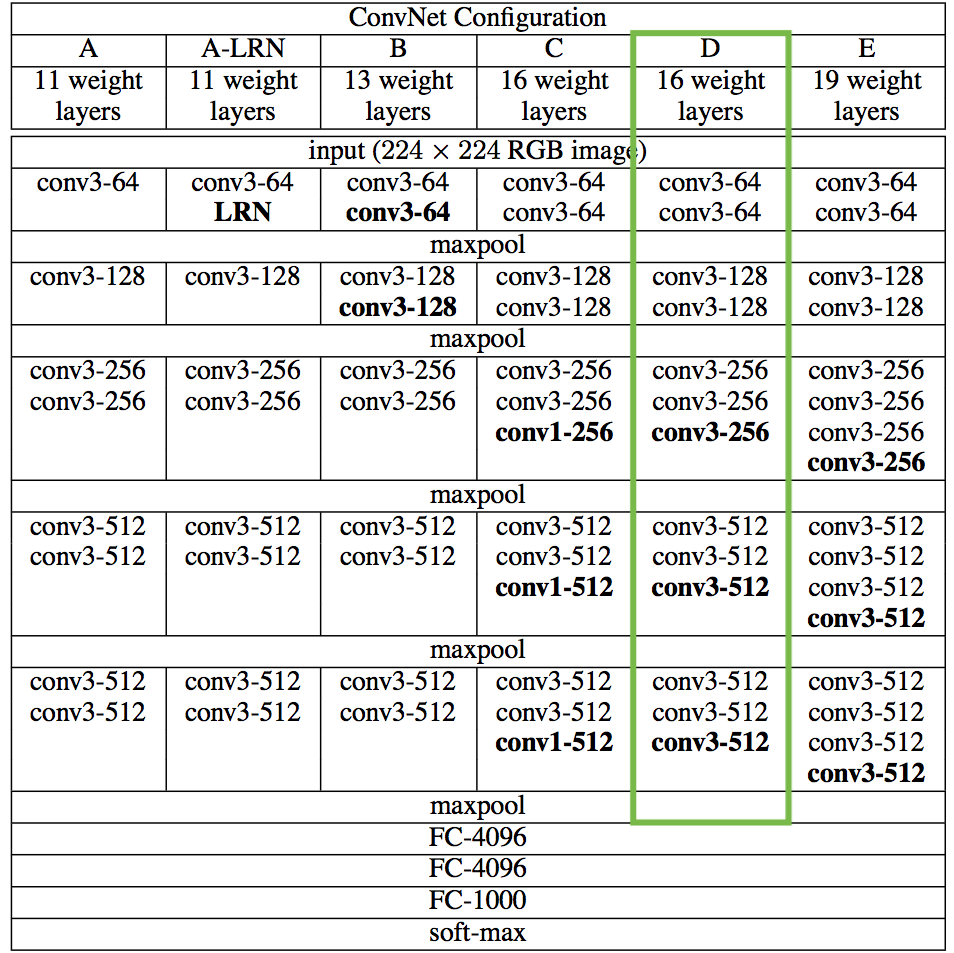
\includegraphics{images/vgg-architecture.png}
\caption{VGG Network Architectures}
\end{figure}

It is trivial for us to get access to this truncated model because Keras
comes with a set of pretrained models, including the VGG16 model we're
interested in. Note that by setting \texttt{include\_top=False} in the
code below, we don't include any of the fully connected layers.

    \begin{Verbatim}[commandchars=\\\{\}]
{\color{incolor}In [{\color{incolor}8}]:} \PY{n}{model} \PY{o}{=} \PY{n}{VGG16}\PY{p}{(}\PY{n}{input\PYZus{}tensor}\PY{o}{=}\PY{n}{input\PYZus{}tensor}\PY{p}{,} \PY{n}{weights}\PY{o}{=}\PY{l+s+s1}{\PYZsq{}}\PY{l+s+s1}{imagenet}\PY{l+s+s1}{\PYZsq{}}\PY{p}{,}
                      \PY{n}{include\PYZus{}top}\PY{o}{=}\PY{k+kc}{False}\PY{p}{)}
\end{Verbatim}


    As is clear from the table above, the model we're working with has a lot
of layers. Keras has its own names for these layers. Let's make a list
of these names so that we can easily refer to individual layers later.

    \begin{Verbatim}[commandchars=\\\{\}]
{\color{incolor}In [{\color{incolor}9}]:} \PY{n}{layers} \PY{o}{=} \PY{n+nb}{dict}\PY{p}{(}\PY{p}{[}\PY{p}{(}\PY{n}{layer}\PY{o}{.}\PY{n}{name}\PY{p}{,} \PY{n}{layer}\PY{o}{.}\PY{n}{output}\PY{p}{)} \PY{k}{for} \PY{n}{layer} \PY{o+ow}{in} \PY{n}{model}\PY{o}{.}\PY{n}{layers}\PY{p}{]}\PY{p}{)}
        \PY{n}{layers}
\end{Verbatim}


\begin{Verbatim}[commandchars=\\\{\}]
{\color{outcolor}Out[{\color{outcolor}9}]:} \{'input\_1': <tf.Tensor 'concat:0' shape=(3, 512, 512, 3) dtype=float32>,
         'block1\_conv1': <tf.Tensor 'block1\_conv1/Relu:0' shape=(3, 512, 512, 64) dtype=float32>,
         'block1\_conv2': <tf.Tensor 'block1\_conv2/Relu:0' shape=(3, 512, 512, 64) dtype=float32>,
         'block1\_pool': <tf.Tensor 'block1\_pool/MaxPool:0' shape=(3, 256, 256, 64) dtype=float32>,
         'block2\_conv1': <tf.Tensor 'block2\_conv1/Relu:0' shape=(3, 256, 256, 128) dtype=float32>,
         'block2\_conv2': <tf.Tensor 'block2\_conv2/Relu:0' shape=(3, 256, 256, 128) dtype=float32>,
         'block2\_pool': <tf.Tensor 'block2\_pool/MaxPool:0' shape=(3, 128, 128, 128) dtype=float32>,
         'block3\_conv1': <tf.Tensor 'block3\_conv1/Relu:0' shape=(3, 128, 128, 256) dtype=float32>,
         'block3\_conv2': <tf.Tensor 'block3\_conv2/Relu:0' shape=(3, 128, 128, 256) dtype=float32>,
         'block3\_conv3': <tf.Tensor 'block3\_conv3/Relu:0' shape=(3, 128, 128, 256) dtype=float32>,
         'block3\_pool': <tf.Tensor 'block3\_pool/MaxPool:0' shape=(3, 64, 64, 256) dtype=float32>,
         'block4\_conv1': <tf.Tensor 'block4\_conv1/Relu:0' shape=(3, 64, 64, 512) dtype=float32>,
         'block4\_conv2': <tf.Tensor 'block4\_conv2/Relu:0' shape=(3, 64, 64, 512) dtype=float32>,
         'block4\_conv3': <tf.Tensor 'block4\_conv3/Relu:0' shape=(3, 64, 64, 512) dtype=float32>,
         'block4\_pool': <tf.Tensor 'block4\_pool/MaxPool:0' shape=(3, 32, 32, 512) dtype=float32>,
         'block5\_conv1': <tf.Tensor 'block5\_conv1/Relu:0' shape=(3, 32, 32, 512) dtype=float32>,
         'block5\_conv2': <tf.Tensor 'block5\_conv2/Relu:0' shape=(3, 32, 32, 512) dtype=float32>,
         'block5\_conv3': <tf.Tensor 'block5\_conv3/Relu:0' shape=(3, 32, 32, 512) dtype=float32>,
         'block5\_pool': <tf.Tensor 'block5\_pool/MaxPool:0' shape=(3, 16, 16, 512) dtype=float32>\}
\end{Verbatim}
            
    If you stare at the list above, you'll convince yourself that we covered
all items we wanted in the table (the cells marked in green). Notice
also that because we provided Keras with a concrete input tensor, the
various TensorFlow tensors get well-defined shapes.

\begin{center}\rule{0.5\linewidth}{\linethickness}\end{center}

The crux of the paper we're trying to reproduce is that the
\href{https://harishnarayanan.org/writing/artistic-style-transfer/}{style
transfer problem can be posed as an optimisation problem}, where the
loss function we want to minimise can be decomposed into three distinct
parts: the \emph{content loss}, the \emph{style loss} and the
\emph{total variation loss}.

The relative importance of these terms are determined by a set of scalar
weights. These are arbitrary, but the following set have been chosen
after quite a bit of experimentation to find a set that generates output
that's aesthetically pleasing to me.

    \begin{Verbatim}[commandchars=\\\{\}]
{\color{incolor}In [{\color{incolor}10}]:} \PY{n}{content\PYZus{}weight} \PY{o}{=} \PY{l+m+mf}{0.025}
         \PY{n}{style\PYZus{}weight} \PY{o}{=} \PY{l+m+mf}{5.0}
         \PY{n}{total\PYZus{}variation\PYZus{}weight} \PY{o}{=} \PY{l+m+mf}{1.0}
\end{Verbatim}


    We'll now use the feature spaces provided by specific layers of our
model to define these three loss functions. We begin by initialising the
total loss to 0 and adding to it in stages.

    \begin{Verbatim}[commandchars=\\\{\}]
{\color{incolor}In [{\color{incolor}11}]:} \PY{n}{loss} \PY{o}{=} \PY{n}{backend}\PY{o}{.}\PY{n}{variable}\PY{p}{(}\PY{l+m+mf}{0.}\PY{p}{)}
\end{Verbatim}


    \subsubsection{The content loss}\label{the-content-loss}

For the content loss, we follow Johnson et al. (2016) and draw the
content feature from \texttt{block2\_conv2}, because the original choice
in Gatys et al. (2015) (\texttt{block4\_conv2}) loses too much
structural detail. And at least for faces, I find it more aesthetically
pleasing to closely retain the structure of the original content image.

This variation across layers is shown for a couple of examples in the
images below (just mentally replace \texttt{reluX\_Y} with our Keras
notation \texttt{blockX\_convY}).

\begin{figure}
\centering
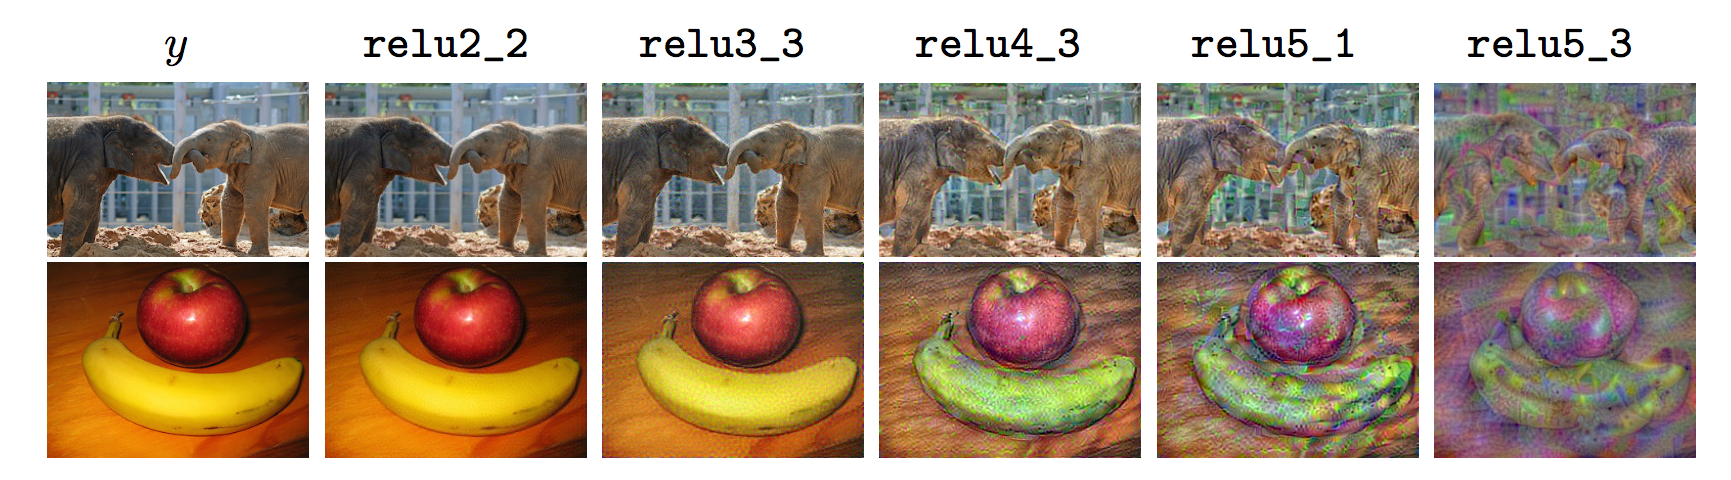
\includegraphics{images/content-feature.png}
\caption{Content feature reconstruction}
\end{figure}

The content loss is the (scaled, squared) Euclidean distance between
feature representations of the content and combination images.

    \begin{Verbatim}[commandchars=\\\{\}]
{\color{incolor}In [{\color{incolor}12}]:} \PY{k}{def} \PY{n+nf}{content\PYZus{}loss}\PY{p}{(}\PY{n}{content}\PY{p}{,} \PY{n}{combination}\PY{p}{)}\PY{p}{:}
             \PY{k}{return} \PY{n}{backend}\PY{o}{.}\PY{n}{sum}\PY{p}{(}\PY{n}{backend}\PY{o}{.}\PY{n}{square}\PY{p}{(}\PY{n}{combination} \PY{o}{\PYZhy{}} \PY{n}{content}\PY{p}{)}\PY{p}{)}
         
         \PY{n}{layer\PYZus{}features} \PY{o}{=} \PY{n}{layers}\PY{p}{[}\PY{l+s+s1}{\PYZsq{}}\PY{l+s+s1}{block2\PYZus{}conv2}\PY{l+s+s1}{\PYZsq{}}\PY{p}{]}
         \PY{n}{content\PYZus{}image\PYZus{}features} \PY{o}{=} \PY{n}{layer\PYZus{}features}\PY{p}{[}\PY{l+m+mi}{0}\PY{p}{,} \PY{p}{:}\PY{p}{,} \PY{p}{:}\PY{p}{,} \PY{p}{:}\PY{p}{]}
         \PY{n}{combination\PYZus{}features} \PY{o}{=} \PY{n}{layer\PYZus{}features}\PY{p}{[}\PY{l+m+mi}{2}\PY{p}{,} \PY{p}{:}\PY{p}{,} \PY{p}{:}\PY{p}{,} \PY{p}{:}\PY{p}{]}
         
         \PY{n}{loss} \PY{o}{+}\PY{o}{=} \PY{n}{content\PYZus{}weight} \PY{o}{*} \PY{n}{content\PYZus{}loss}\PY{p}{(}\PY{n}{content\PYZus{}image\PYZus{}features}\PY{p}{,}
                                               \PY{n}{combination\PYZus{}features}\PY{p}{)}
\end{Verbatim}


    \begin{Verbatim}[commandchars=\\\{\}]
WARNING:tensorflow:Variable += will be deprecated. Use variable.assign\_add if you want assignment to the variable value or 'x = x + y' if you want a new python Tensor object.

    \end{Verbatim}

    \subsubsection{The style loss}\label{the-style-loss}

This is where things start to get a bit intricate.

For the style loss, we first define something called a \emph{Gram
matrix}. The terms of this matrix are proportional to the covariances of
corresponding sets of features, and thus captures information about
which features tend to activate together. By only capturing these
aggregate statistics across the image, they are blind to the specific
arrangement of objects inside the image. This is what allows them to
capture information about style independent of content. (This is not
trivial at all, and I refer you to
\href{https://arxiv.org/abs/1606.01286}{a paper that attempts to explain
the idea}.)

The Gram matrix can be computed efficiently by reshaping the feature
spaces suitably and taking an outer product.

    \begin{Verbatim}[commandchars=\\\{\}]
{\color{incolor}In [{\color{incolor}13}]:} \PY{k}{def} \PY{n+nf}{gram\PYZus{}matrix}\PY{p}{(}\PY{n}{x}\PY{p}{)}\PY{p}{:}
             \PY{n}{features} \PY{o}{=} \PY{n}{backend}\PY{o}{.}\PY{n}{batch\PYZus{}flatten}\PY{p}{(}\PY{n}{backend}\PY{o}{.}\PY{n}{permute\PYZus{}dimensions}\PY{p}{(}\PY{n}{x}\PY{p}{,} \PY{p}{(}\PY{l+m+mi}{2}\PY{p}{,} \PY{l+m+mi}{0}\PY{p}{,} \PY{l+m+mi}{1}\PY{p}{)}\PY{p}{)}\PY{p}{)}
             \PY{n}{gram} \PY{o}{=} \PY{n}{backend}\PY{o}{.}\PY{n}{dot}\PY{p}{(}\PY{n}{features}\PY{p}{,} \PY{n}{backend}\PY{o}{.}\PY{n}{transpose}\PY{p}{(}\PY{n}{features}\PY{p}{)}\PY{p}{)}
             \PY{k}{return} \PY{n}{gram}
\end{Verbatim}


    The style loss is then the (scaled, squared) Frobenius norm of the
difference between the Gram matrices of the style and combination
images.

Again, in the following code, I've chosen to go with the style features
from layers defined in Johnson et al. (2016) rather than Gatys et al.
(2015) because I find the end results more aesthetically pleasing. I
encourage you to experiment with these choices to see varying results.

    \begin{Verbatim}[commandchars=\\\{\}]
{\color{incolor}In [{\color{incolor}14}]:} \PY{k}{def} \PY{n+nf}{style\PYZus{}loss}\PY{p}{(}\PY{n}{style}\PY{p}{,} \PY{n}{combination}\PY{p}{)}\PY{p}{:}
             \PY{n}{S} \PY{o}{=} \PY{n}{gram\PYZus{}matrix}\PY{p}{(}\PY{n}{style}\PY{p}{)}
             \PY{n}{C} \PY{o}{=} \PY{n}{gram\PYZus{}matrix}\PY{p}{(}\PY{n}{combination}\PY{p}{)}
             \PY{n}{channels} \PY{o}{=} \PY{l+m+mi}{3}
             \PY{n}{size} \PY{o}{=} \PY{n}{height} \PY{o}{*} \PY{n}{width}
             \PY{k}{return} \PY{n}{backend}\PY{o}{.}\PY{n}{sum}\PY{p}{(}\PY{n}{backend}\PY{o}{.}\PY{n}{square}\PY{p}{(}\PY{n}{S} \PY{o}{\PYZhy{}} \PY{n}{C}\PY{p}{)}\PY{p}{)} \PY{o}{/} \PY{p}{(}\PY{l+m+mf}{4.} \PY{o}{*} \PY{p}{(}\PY{n}{channels} \PY{o}{*}\PY{o}{*} \PY{l+m+mi}{2}\PY{p}{)} \PY{o}{*} \PY{p}{(}\PY{n}{size} \PY{o}{*}\PY{o}{*} \PY{l+m+mi}{2}\PY{p}{)}\PY{p}{)}
         
         \PY{n}{feature\PYZus{}layers} \PY{o}{=} \PY{p}{[}\PY{l+s+s1}{\PYZsq{}}\PY{l+s+s1}{block1\PYZus{}conv2}\PY{l+s+s1}{\PYZsq{}}\PY{p}{,} \PY{l+s+s1}{\PYZsq{}}\PY{l+s+s1}{block2\PYZus{}conv2}\PY{l+s+s1}{\PYZsq{}}\PY{p}{,}
                           \PY{l+s+s1}{\PYZsq{}}\PY{l+s+s1}{block3\PYZus{}conv3}\PY{l+s+s1}{\PYZsq{}}\PY{p}{,} \PY{l+s+s1}{\PYZsq{}}\PY{l+s+s1}{block4\PYZus{}conv3}\PY{l+s+s1}{\PYZsq{}}\PY{p}{,}
                           \PY{l+s+s1}{\PYZsq{}}\PY{l+s+s1}{block5\PYZus{}conv3}\PY{l+s+s1}{\PYZsq{}}\PY{p}{]}
         \PY{k}{for} \PY{n}{layer\PYZus{}name} \PY{o+ow}{in} \PY{n}{feature\PYZus{}layers}\PY{p}{:}
             \PY{n}{layer\PYZus{}features} \PY{o}{=} \PY{n}{layers}\PY{p}{[}\PY{n}{layer\PYZus{}name}\PY{p}{]}
             \PY{n}{style\PYZus{}features} \PY{o}{=} \PY{n}{layer\PYZus{}features}\PY{p}{[}\PY{l+m+mi}{1}\PY{p}{,} \PY{p}{:}\PY{p}{,} \PY{p}{:}\PY{p}{,} \PY{p}{:}\PY{p}{]}
             \PY{n}{combination\PYZus{}features} \PY{o}{=} \PY{n}{layer\PYZus{}features}\PY{p}{[}\PY{l+m+mi}{2}\PY{p}{,} \PY{p}{:}\PY{p}{,} \PY{p}{:}\PY{p}{,} \PY{p}{:}\PY{p}{]}
             \PY{n}{sl} \PY{o}{=} \PY{n}{style\PYZus{}loss}\PY{p}{(}\PY{n}{style\PYZus{}features}\PY{p}{,} \PY{n}{combination\PYZus{}features}\PY{p}{)}
             \PY{n}{loss} \PY{o}{+}\PY{o}{=} \PY{p}{(}\PY{n}{style\PYZus{}weight} \PY{o}{/} \PY{n+nb}{len}\PY{p}{(}\PY{n}{feature\PYZus{}layers}\PY{p}{)}\PY{p}{)} \PY{o}{*} \PY{n}{sl}
\end{Verbatim}


    \subsubsection{The total variation loss}\label{the-total-variation-loss}

Now we're back on simpler ground.

If you were to solve the optimisation problem with only the two loss
terms we've introduced so far (style and content), you'll find that the
output is quite noisy. We thus add another term, called the
\href{http://arxiv.org/abs/1412.0035}{total variation loss} (a
regularisation term) that encourages spatial smoothness.

You can experiment with reducing the \texttt{total\_variation\_weight}
and play with the noise-level of the generated image.

    \begin{Verbatim}[commandchars=\\\{\}]
{\color{incolor}In [{\color{incolor}15}]:} \PY{k}{def} \PY{n+nf}{total\PYZus{}variation\PYZus{}loss}\PY{p}{(}\PY{n}{x}\PY{p}{)}\PY{p}{:}
             \PY{n}{a} \PY{o}{=} \PY{n}{backend}\PY{o}{.}\PY{n}{square}\PY{p}{(}\PY{n}{x}\PY{p}{[}\PY{p}{:}\PY{p}{,} \PY{p}{:}\PY{n}{height}\PY{o}{\PYZhy{}}\PY{l+m+mi}{1}\PY{p}{,} \PY{p}{:}\PY{n}{width}\PY{o}{\PYZhy{}}\PY{l+m+mi}{1}\PY{p}{,} \PY{p}{:}\PY{p}{]} \PY{o}{\PYZhy{}} \PY{n}{x}\PY{p}{[}\PY{p}{:}\PY{p}{,} \PY{l+m+mi}{1}\PY{p}{:}\PY{p}{,} \PY{p}{:}\PY{n}{width}\PY{o}{\PYZhy{}}\PY{l+m+mi}{1}\PY{p}{,} \PY{p}{:}\PY{p}{]}\PY{p}{)}
             \PY{n}{b} \PY{o}{=} \PY{n}{backend}\PY{o}{.}\PY{n}{square}\PY{p}{(}\PY{n}{x}\PY{p}{[}\PY{p}{:}\PY{p}{,} \PY{p}{:}\PY{n}{height}\PY{o}{\PYZhy{}}\PY{l+m+mi}{1}\PY{p}{,} \PY{p}{:}\PY{n}{width}\PY{o}{\PYZhy{}}\PY{l+m+mi}{1}\PY{p}{,} \PY{p}{:}\PY{p}{]} \PY{o}{\PYZhy{}} \PY{n}{x}\PY{p}{[}\PY{p}{:}\PY{p}{,} \PY{p}{:}\PY{n}{height}\PY{o}{\PYZhy{}}\PY{l+m+mi}{1}\PY{p}{,} \PY{l+m+mi}{1}\PY{p}{:}\PY{p}{,} \PY{p}{:}\PY{p}{]}\PY{p}{)}
             \PY{k}{return} \PY{n}{backend}\PY{o}{.}\PY{n}{sum}\PY{p}{(}\PY{n}{backend}\PY{o}{.}\PY{n}{pow}\PY{p}{(}\PY{n}{a} \PY{o}{+} \PY{n}{b}\PY{p}{,} \PY{l+m+mf}{1.25}\PY{p}{)}\PY{p}{)}
         
         \PY{n}{loss} \PY{o}{+}\PY{o}{=} \PY{n}{total\PYZus{}variation\PYZus{}weight} \PY{o}{*} \PY{n}{total\PYZus{}variation\PYZus{}loss}\PY{p}{(}\PY{n}{combination\PYZus{}image}\PY{p}{)}
\end{Verbatim}


    \subsection{Define needed gradients and solve the optimisation
problem}\label{define-needed-gradients-and-solve-the-optimisation-problem}

\href{https://harishnarayanan.org/writing/artistic-style-transfer/}{The
goal of this journey} was to setup an optimisation problem that aims to
solve for a \emph{combination image} that contains the content of the
content image, while having the style of the style image. Now that we
have our input images massaged and our loss function calculators in
place, all we have left to do is define gradients of the total loss
relative to the combination image, and use these gradients to
iteratively improve upon our combination image to minimise the loss.

We start by defining the gradients.

    \begin{Verbatim}[commandchars=\\\{\}]
{\color{incolor}In [{\color{incolor}16}]:} \PY{n}{grads} \PY{o}{=} \PY{n}{backend}\PY{o}{.}\PY{n}{gradients}\PY{p}{(}\PY{n}{loss}\PY{p}{,} \PY{n}{combination\PYZus{}image}\PY{p}{)}
\end{Verbatim}


    We then introduce an \texttt{Evaluator} class that computes loss and
gradients in one pass while retrieving them via two separate functions,
\texttt{loss} and \texttt{grads}. This is done because
\texttt{scipy.optimize} requires separate functions for loss and
gradients, but computing them separately would be inefficient.

    \begin{Verbatim}[commandchars=\\\{\}]
{\color{incolor}In [{\color{incolor}17}]:} \PY{n}{outputs} \PY{o}{=} \PY{p}{[}\PY{n}{loss}\PY{p}{]}
         \PY{n}{outputs} \PY{o}{+}\PY{o}{=} \PY{n}{grads}
         \PY{n}{f\PYZus{}outputs} \PY{o}{=} \PY{n}{backend}\PY{o}{.}\PY{n}{function}\PY{p}{(}\PY{p}{[}\PY{n}{combination\PYZus{}image}\PY{p}{]}\PY{p}{,} \PY{n}{outputs}\PY{p}{)}
         
         \PY{k}{def} \PY{n+nf}{eval\PYZus{}loss\PYZus{}and\PYZus{}grads}\PY{p}{(}\PY{n}{x}\PY{p}{)}\PY{p}{:}
             \PY{n}{x} \PY{o}{=} \PY{n}{x}\PY{o}{.}\PY{n}{reshape}\PY{p}{(}\PY{p}{(}\PY{l+m+mi}{1}\PY{p}{,} \PY{n}{height}\PY{p}{,} \PY{n}{width}\PY{p}{,} \PY{l+m+mi}{3}\PY{p}{)}\PY{p}{)}
             \PY{n}{outs} \PY{o}{=} \PY{n}{f\PYZus{}outputs}\PY{p}{(}\PY{p}{[}\PY{n}{x}\PY{p}{]}\PY{p}{)}
             \PY{n}{loss\PYZus{}value} \PY{o}{=} \PY{n}{outs}\PY{p}{[}\PY{l+m+mi}{0}\PY{p}{]}
             \PY{n}{grad\PYZus{}values} \PY{o}{=} \PY{n}{outs}\PY{p}{[}\PY{l+m+mi}{1}\PY{p}{]}\PY{o}{.}\PY{n}{flatten}\PY{p}{(}\PY{p}{)}\PY{o}{.}\PY{n}{astype}\PY{p}{(}\PY{l+s+s1}{\PYZsq{}}\PY{l+s+s1}{float64}\PY{l+s+s1}{\PYZsq{}}\PY{p}{)}
             \PY{k}{return} \PY{n}{loss\PYZus{}value}\PY{p}{,} \PY{n}{grad\PYZus{}values}
         
         \PY{k}{class} \PY{n+nc}{Evaluator}\PY{p}{(}\PY{n+nb}{object}\PY{p}{)}\PY{p}{:}
         
             \PY{k}{def} \PY{n+nf}{\PYZus{}\PYZus{}init\PYZus{}\PYZus{}}\PY{p}{(}\PY{n+nb+bp}{self}\PY{p}{)}\PY{p}{:}
                 \PY{n+nb+bp}{self}\PY{o}{.}\PY{n}{loss\PYZus{}value} \PY{o}{=} \PY{k+kc}{None}
                 \PY{n+nb+bp}{self}\PY{o}{.}\PY{n}{grads\PYZus{}values} \PY{o}{=} \PY{k+kc}{None}
         
             \PY{k}{def} \PY{n+nf}{loss}\PY{p}{(}\PY{n+nb+bp}{self}\PY{p}{,} \PY{n}{x}\PY{p}{)}\PY{p}{:}
                 \PY{k}{assert} \PY{n+nb+bp}{self}\PY{o}{.}\PY{n}{loss\PYZus{}value} \PY{o+ow}{is} \PY{k+kc}{None}
                 \PY{n}{loss\PYZus{}value}\PY{p}{,} \PY{n}{grad\PYZus{}values} \PY{o}{=} \PY{n}{eval\PYZus{}loss\PYZus{}and\PYZus{}grads}\PY{p}{(}\PY{n}{x}\PY{p}{)}
                 \PY{n+nb+bp}{self}\PY{o}{.}\PY{n}{loss\PYZus{}value} \PY{o}{=} \PY{n}{loss\PYZus{}value}
                 \PY{n+nb+bp}{self}\PY{o}{.}\PY{n}{grad\PYZus{}values} \PY{o}{=} \PY{n}{grad\PYZus{}values}
                 \PY{k}{return} \PY{n+nb+bp}{self}\PY{o}{.}\PY{n}{loss\PYZus{}value}
         
             \PY{k}{def} \PY{n+nf}{grads}\PY{p}{(}\PY{n+nb+bp}{self}\PY{p}{,} \PY{n}{x}\PY{p}{)}\PY{p}{:}
                 \PY{k}{assert} \PY{n+nb+bp}{self}\PY{o}{.}\PY{n}{loss\PYZus{}value} \PY{o+ow}{is} \PY{o+ow}{not} \PY{k+kc}{None}
                 \PY{n}{grad\PYZus{}values} \PY{o}{=} \PY{n}{np}\PY{o}{.}\PY{n}{copy}\PY{p}{(}\PY{n+nb+bp}{self}\PY{o}{.}\PY{n}{grad\PYZus{}values}\PY{p}{)}
                 \PY{n+nb+bp}{self}\PY{o}{.}\PY{n}{loss\PYZus{}value} \PY{o}{=} \PY{k+kc}{None}
                 \PY{n+nb+bp}{self}\PY{o}{.}\PY{n}{grad\PYZus{}values} \PY{o}{=} \PY{k+kc}{None}
                 \PY{k}{return} \PY{n}{grad\PYZus{}values}
         
         \PY{n}{evaluator} \PY{o}{=} \PY{n}{Evaluator}\PY{p}{(}\PY{p}{)}
\end{Verbatim}


    Now we're finally ready to solve our optimisation problem. This
combination image begins its life as a random collection of (valid)
pixels, and we use the
\href{https://en.wikipedia.org/wiki/Limited-memory_BFGS}{L-BFGS}
algorithm (a quasi-Newton algorithm that's significantly quicker to
converge than standard gradient descent) to iteratively improve upon it.

We stop after 10 iterations because the output looks good to me and the
loss stops reducing significantly.

    \begin{Verbatim}[commandchars=\\\{\}]
{\color{incolor}In [{\color{incolor}18}]:} \PY{n}{x} \PY{o}{=} \PY{n}{np}\PY{o}{.}\PY{n}{random}\PY{o}{.}\PY{n}{uniform}\PY{p}{(}\PY{l+m+mi}{0}\PY{p}{,} \PY{l+m+mi}{255}\PY{p}{,} \PY{p}{(}\PY{l+m+mi}{1}\PY{p}{,} \PY{n}{height}\PY{p}{,} \PY{n}{width}\PY{p}{,} \PY{l+m+mi}{3}\PY{p}{)}\PY{p}{)} \PY{o}{\PYZhy{}} \PY{l+m+mf}{128.}
         
         \PY{n}{iterations} \PY{o}{=} \PY{l+m+mi}{10}
         
         \PY{k}{for} \PY{n}{i} \PY{o+ow}{in} \PY{n+nb}{range}\PY{p}{(}\PY{n}{iterations}\PY{p}{)}\PY{p}{:}
             \PY{n+nb}{print}\PY{p}{(}\PY{l+s+s1}{\PYZsq{}}\PY{l+s+s1}{Start of iteration}\PY{l+s+s1}{\PYZsq{}}\PY{p}{,} \PY{n}{i}\PY{p}{)}
             
             \PY{n}{start\PYZus{}time} \PY{o}{=} \PY{n}{time}\PY{o}{.}\PY{n}{time}\PY{p}{(}\PY{p}{)}
             \PY{n}{x}\PY{p}{,} \PY{n}{min\PYZus{}val}\PY{p}{,} \PY{n}{info} \PY{o}{=} \PY{n}{fmin\PYZus{}l\PYZus{}bfgs\PYZus{}b}\PY{p}{(}\PY{n}{evaluator}\PY{o}{.}\PY{n}{loss}\PY{p}{,} \PY{n}{x}\PY{o}{.}\PY{n}{flatten}\PY{p}{(}\PY{p}{)}\PY{p}{,}
                                              \PY{n}{fprime}\PY{o}{=}\PY{n}{evaluator}\PY{o}{.}\PY{n}{grads}\PY{p}{,} \PY{n}{maxfun}\PY{o}{=}\PY{l+m+mi}{20}\PY{p}{)}
             \PY{n+nb}{print}\PY{p}{(}\PY{l+s+s1}{\PYZsq{}}\PY{l+s+s1}{Current loss value:}\PY{l+s+s1}{\PYZsq{}}\PY{p}{,} \PY{n}{min\PYZus{}val}\PY{p}{)}
             \PY{n}{end\PYZus{}time} \PY{o}{=} \PY{n}{time}\PY{o}{.}\PY{n}{time}\PY{p}{(}\PY{p}{)}
             \PY{n+nb}{print}\PY{p}{(}\PY{l+s+s1}{\PYZsq{}}\PY{l+s+s1}{Iteration }\PY{l+s+si}{\PYZpc{}d}\PY{l+s+s1}{ completed in }\PY{l+s+si}{\PYZpc{}d}\PY{l+s+s1}{s}\PY{l+s+s1}{\PYZsq{}} \PY{o}{\PYZpc{}} \PY{p}{(}\PY{n}{i}\PY{p}{,} \PY{n}{end\PYZus{}time} \PY{o}{\PYZhy{}} \PY{n}{start\PYZus{}time}\PY{p}{)}\PY{p}{)}
\end{Verbatim}


    \begin{Verbatim}[commandchars=\\\{\}]
Start of iteration 0
Current loss value: 77721350000.0
Iteration 0 completed in 317s
Start of iteration 1
Current loss value: 54563693000.0
Iteration 1 completed in 319s
Start of iteration 2
Current loss value: 43882316000.0
Iteration 2 completed in 324s
Start of iteration 3
Current loss value: 39966212000.0
Iteration 3 completed in 331s
Start of iteration 4
Current loss value: 38282620000.0
Iteration 4 completed in 328s
Start of iteration 5
Current loss value: 37246562000.0
Iteration 5 completed in 299s
Start of iteration 6
Current loss value: 36617617000.0
Iteration 6 completed in 298s
Start of iteration 7
Current loss value: 36182483000.0
Iteration 7 completed in 302s
Start of iteration 8
Current loss value: 35898364000.0
Iteration 8 completed in 304s
Start of iteration 9
Current loss value: 35701190000.0
Iteration 9 completed in 300s

    \end{Verbatim}

    This took a while on my piddly laptop (that isn't GPU-accelerated), but
here is the beautiful output from the last iteration! (Notice that we
need to subject our output image to the inverse of the transformation we
did to our input images before it makes sense.)

    \begin{Verbatim}[commandchars=\\\{\}]
{\color{incolor}In [{\color{incolor}19}]:} \PY{n}{x} \PY{o}{=} \PY{n}{x}\PY{o}{.}\PY{n}{reshape}\PY{p}{(}\PY{p}{(}\PY{n}{height}\PY{p}{,} \PY{n}{width}\PY{p}{,} \PY{l+m+mi}{3}\PY{p}{)}\PY{p}{)}
         \PY{n}{x} \PY{o}{=} \PY{n}{x}\PY{p}{[}\PY{p}{:}\PY{p}{,} \PY{p}{:}\PY{p}{,} \PY{p}{:}\PY{p}{:}\PY{o}{\PYZhy{}}\PY{l+m+mi}{1}\PY{p}{]}
         \PY{n}{x}\PY{p}{[}\PY{p}{:}\PY{p}{,} \PY{p}{:}\PY{p}{,} \PY{l+m+mi}{0}\PY{p}{]} \PY{o}{+}\PY{o}{=} \PY{l+m+mf}{103.939}
         \PY{n}{x}\PY{p}{[}\PY{p}{:}\PY{p}{,} \PY{p}{:}\PY{p}{,} \PY{l+m+mi}{1}\PY{p}{]} \PY{o}{+}\PY{o}{=} \PY{l+m+mf}{116.779}
         \PY{n}{x}\PY{p}{[}\PY{p}{:}\PY{p}{,} \PY{p}{:}\PY{p}{,} \PY{l+m+mi}{2}\PY{p}{]} \PY{o}{+}\PY{o}{=} \PY{l+m+mf}{123.68}
         \PY{n}{x} \PY{o}{=} \PY{n}{np}\PY{o}{.}\PY{n}{clip}\PY{p}{(}\PY{n}{x}\PY{p}{,} \PY{l+m+mi}{0}\PY{p}{,} \PY{l+m+mi}{255}\PY{p}{)}\PY{o}{.}\PY{n}{astype}\PY{p}{(}\PY{l+s+s1}{\PYZsq{}}\PY{l+s+s1}{uint8}\PY{l+s+s1}{\PYZsq{}}\PY{p}{)}
         
         \PY{n}{Image}\PY{o}{.}\PY{n}{fromarray}\PY{p}{(}\PY{n}{x}\PY{p}{)}
\end{Verbatim}

\texttt{\color{outcolor}Out[{\color{outcolor}19}]:}
    
    \begin{center}
    \adjustimage{max size={0.9\linewidth}{0.9\paperheight}}{output_36_0.png}
    \end{center}
    { \hspace*{\fill} \\}
    

    \subsection{Conclusion and further
improvements}\label{conclusion-and-further-improvements}

It's now your turn to play! Try changing the input images, their sizes,
the weights of the different loss functions, the features used to
construct them and enjoy different sorts of output. If you end up
creating something you truly wish to share,
\href{https://twitter.com/copingbear}{please do so}!

As beautiful as the output of this code can be, the process we use to
generate it is quite slow. And no matter how much you speed this
algorithm up (with GPUs and creative hacks), it is still going to be a
relatively expensive problem to solve. This is because we're solving an
entire optimisation problem each time we want to generate an image.

In an upcoming article (and corresponding iPython notebook), we're going
to replace this the optimisation problem with an image transformation
CNN, which in turn uses the VGG16 network as before to measure losses.
When this transformation network is trained on many images given a fixed
style image, we end up with a fully feed-forward CNN that we can apply
for style transfer. This gives us a 1000x speed up over this
implementation, making it suitable for a the \emph{Stylist} webapp.

But more on that later.


    % Add a bibliography block to the postdoc
    
    
    
    \end{document}
